
%: ----------------------- introduction file header -----------------------


% the code below specifies where the figures are stored
\ifpdf
    \graphicspath{{introduction/figures/PNG/}{introduction/figures/PDF/}{introduction/figures/}}
\else
    \graphicspath{{introduction/figures/EPS/}{introduction/figures/}}
\fi

% ----------------------------------------------------------------------
%: ----------------------- introduction content ----------------------- 
% ----------------------------------------------------------------------
\chapter{First Things First}
\section{Cosmic Context}\label{sec:CosmicContext}


Oh, you know, stars 'n' stuff.

\section{The Shoulders of Giants} 

Before we begin, it is first worth appreciating the difficulty of what we are trying to do. Essentially, we care about measuring the properties of the intergalactic gas -- not stars or galaxies -- when the Universe was only $\sim$1 billion years old, a seemingly impossible task. Fortunately, we are given the invaluable gift that light travels at a finite speed and, as such, if we look at distant objects, we see them as they were in the past. Therefore, if we look at the at the gas between galaxies $\sim$13 billion light years away from us, we will see it as it was roughly 13 billion years ago, when the Universe was only 1 billion years old. This means that, in principle, this information of how the young IGM evolved is directly available to us. However, even taking this into account, the intergalactic gas we care about is not bright and it is located $\text{extremely}^{\text{extremely}}$ far away, so how are we supposed to observe it? An exciting aspect of studying the Epoch of Reionization is that, when confronted with such a seemingly impossible task, experts in the field have developed many different creative approaches toward constraining the properties of the young IGM in order to learn about the Epoch of Reionization. It is this impressive body of work that we aim to build upon. We discuss a selection of the existing and future methods for constraining the EoR in this chapter.

\subsection{The \lya\ Forest}
Arguably the most powerful tool for constraining the high-redshift IGM to date has been the \lya\ forest\nomenclature[Zp]{\lya\ Forest}{This describes the pattern of absorption lines seen blueward of the rest-frame \lya\ line, typically in quasar spectra. These absorption lines can be due to significantly neutral gas in the diffuse IGM or due to dense ionized gas.}. The \lya\ forest results, in part, from another invaluable gift to the field of cosmology: the redshifting of light with the expansion of the Universe. Basically, as the Universe expands, space itself expands and with it the wavelengths of photons travelling through it expand as well. If we know the expansion history of the Universe, and know the intrinsic color of a luminous object, then we can use its \textit{observed} color to determine our distance to the object. Because of this relationship, distances to objects are often measured as a redshift\nomenclature[Zp]{Redshift}{A quantity commonly used to refer to cosmic periods of time or distances. The redshift of an object or location in space is defined as the fractional increase in wavelength that a photon undergoes due to the expansion of the Universe while travelling from the object or location to us.}, defined as the fractional increase in wavelength that a photon experiences when travelling from a given distance to us, denoted by $z$. In other ``words": 

\begin{align}
\lambda_{\text{observed}} &= \lambda_{\text{emitted}}(1+z_{\text{emitter}}). 
\end{align}

The \lya\ forest can be seen in the spectrum of an extremely bright background object, usually a quasar\nomenclature[Zp]{Quasar}{It's bright, OK?} or a gamma-ray burst (GRB)\nomenclature[Zp]{GRB}{Gamma-Ray Burst. They are also really bright, OK?}, after its light has been processed by the intervening gas. Since the intervening gas is primarily composed of hydrogen and since this hydrogen is generally in the ground state, any intervening neutral patches will absorb light from the background object at the Lyman-series wavelengths, with the strongest absorption occurring at the \lya\ wavelength: $\lambda_{\alpha} \approx 1216$\AA. If the Universe were not expanding, then all intervening neutral hydrogen would absorb light from the quasar at one wavelength: $\lambda_{\alpha} \approx 1216$\angstrom, neglecting the other lines in the Lyman-series for the moment. However, due to the expansion of the Universe, photons emitted from the quasar \textit{blueward} of the \lya\ line will redshift as they travel towards us. If they encounter neutral hydrogen as they redshift through the \lya\ line, then they will be absorbed and an absorption line will be seen in the spectrum of the background quasar at a wavelength \textit{blueward} of \lya. This process is sketched in Figure \ref{fig:LyaCartoon}. Thus, the \lya\ forest is the pattern of absorption lines seen blueward of the rest-frame \lya\ line in quasar spectra due to intervening neutral gas. 

\begin{figure}[h]
  \centering
  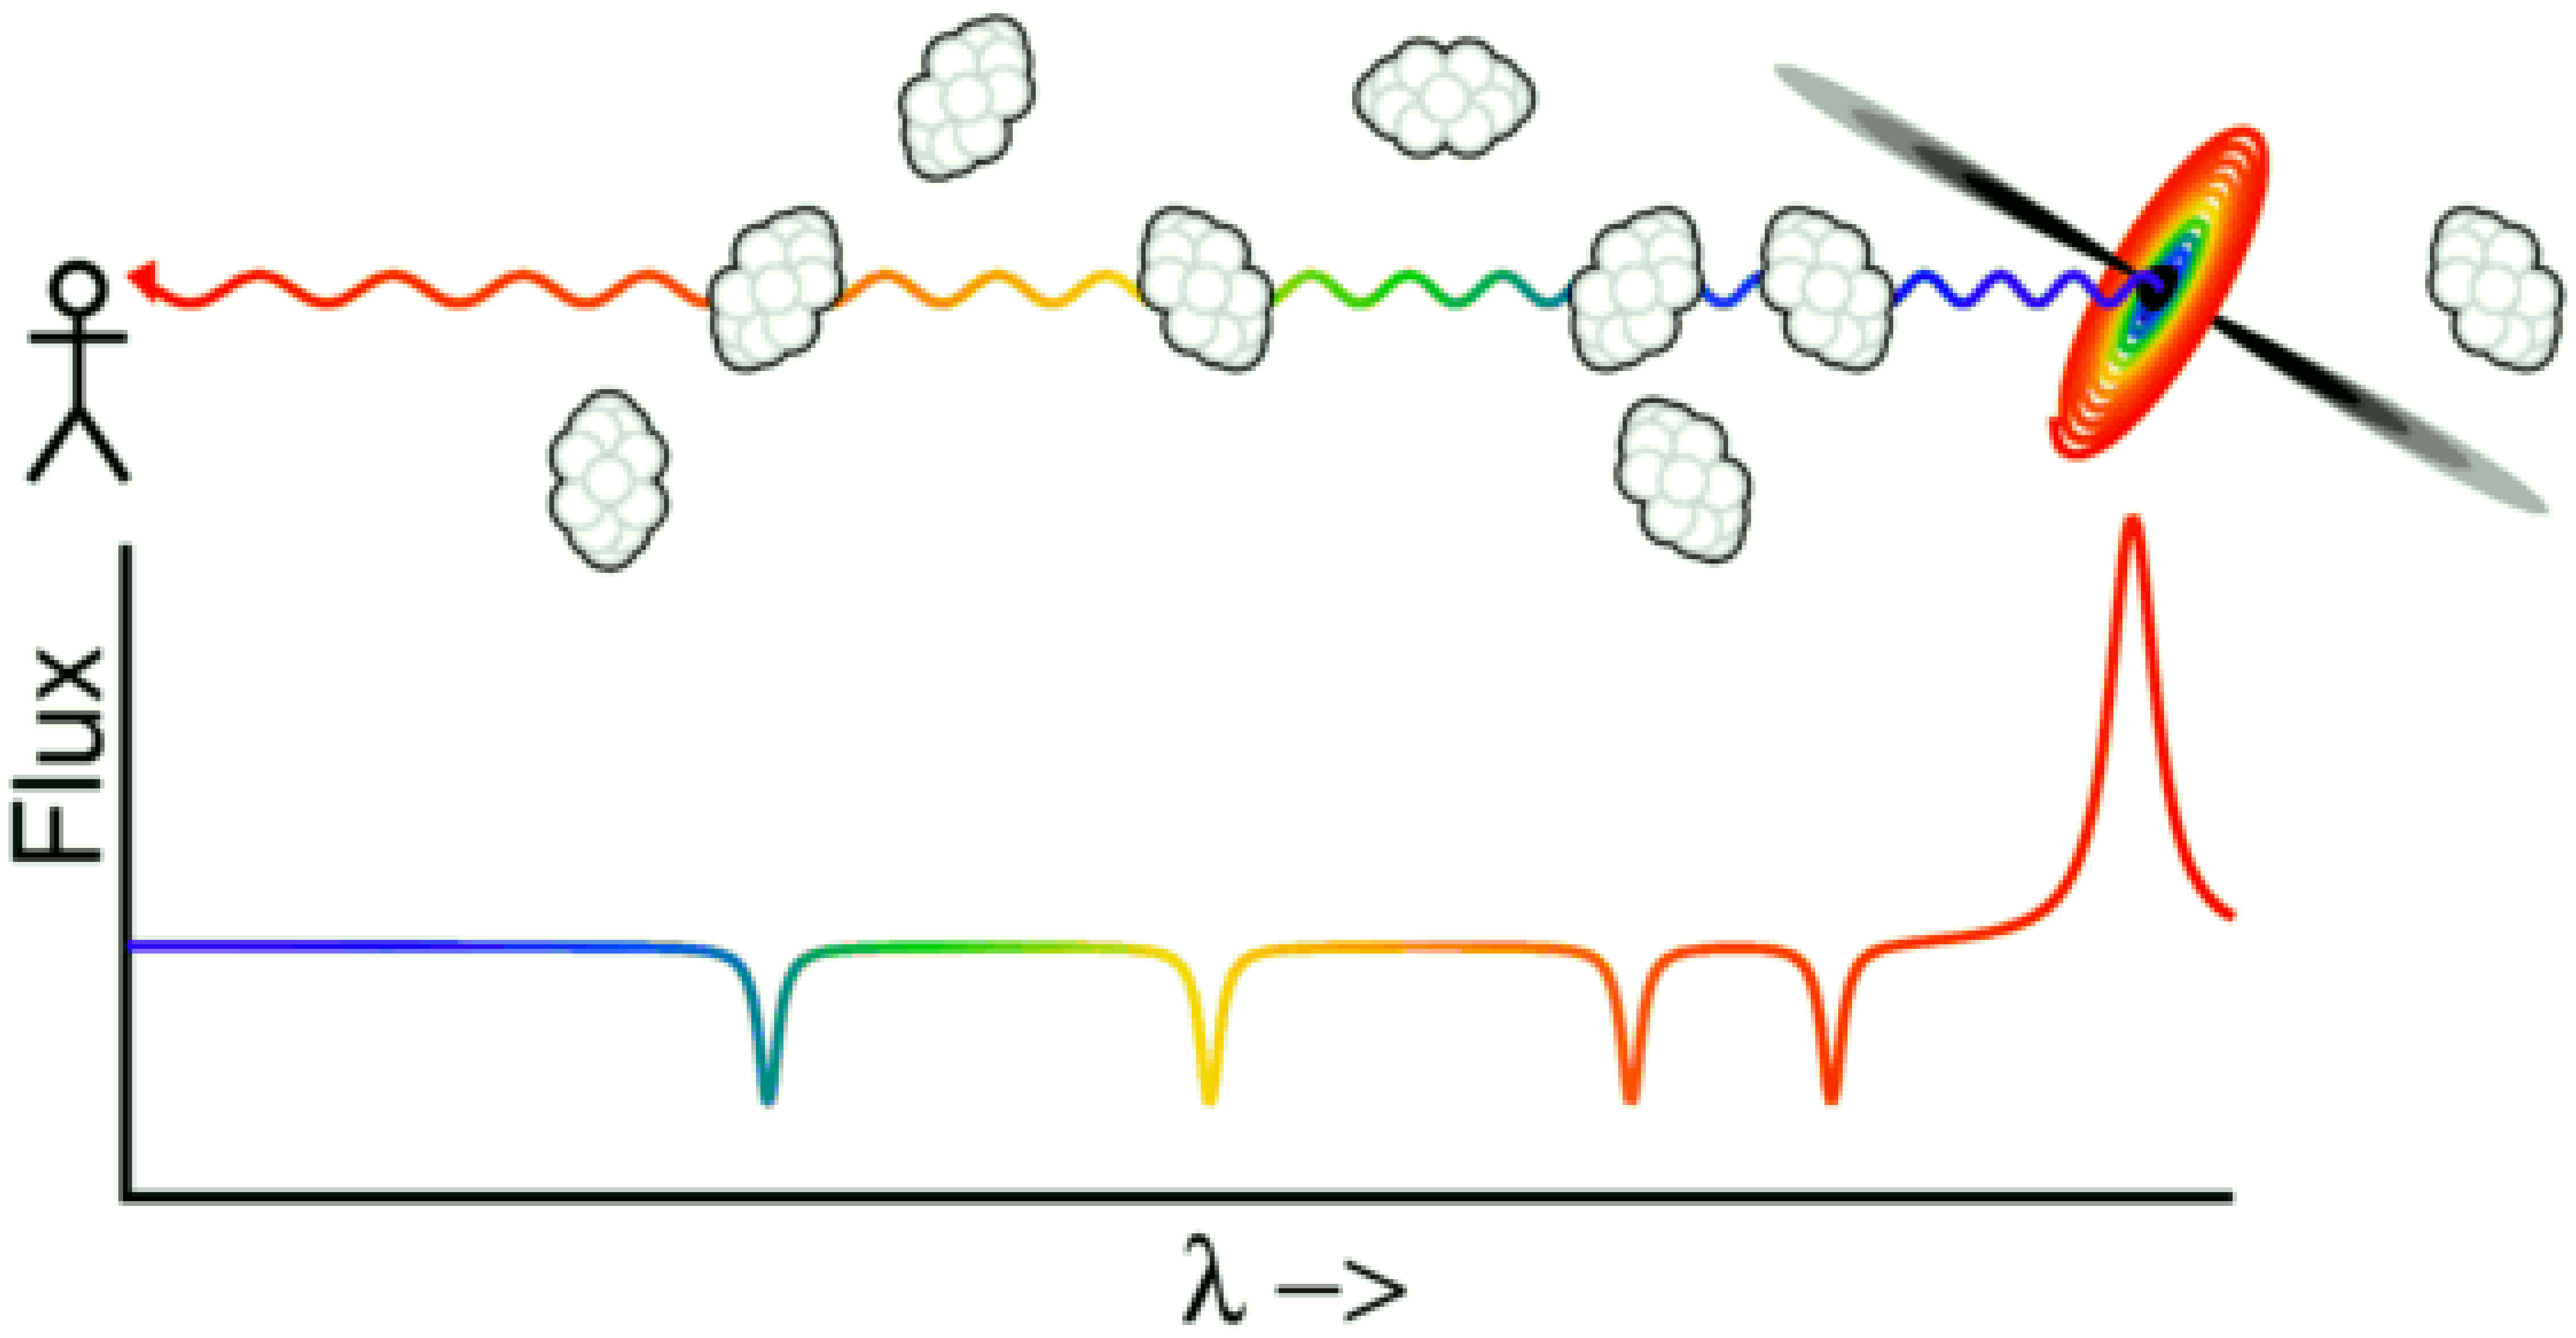
\includegraphics[width=12cm]{lyaf-75.eps}
  \caption{Illustration of the basic physics behind the \lya\ forest and how gas at different locations along the line of sight results in absorption lines at different wavelengths. (Image from {\tt http://www.astro.ucla.edu/})}
  \label{fig:LyaCartoon}
\end{figure}

The same logical progression also applies to the other lines in the Lyman-series, with the difference that lines deeper in the series have a smaller cross section for absorption. Therefore, you could imagine observing a \lyb\ and Ly\ $\gamma$\ forest at smaller wavelengths. Another important difference here, though, is that photons emitted from a background source with energies larger than \lyb\ will redshift through the \lyb\ wavelength and \textit{also} possibly through the \lya\ wavelength before reaching us. The photon's physical location when it redshifts through those two wavelengths will be completely different and, therefore, when observing absorption lines in the \lyb\ forest, it can be difficult to tell if the photons were absorbed by distant gas undergoing a \lyb\ transmission or closer gas undergoing a \lya\ transition. This problem is clearly exacerbated when considering higher-order lines since a larger number of distinct regions along the line of sight can contribute to the absorption.


We show two example quasar spectra in Figure \ref{fig:LyaExample}. The spectrum in the top panel is for a quasar at relatively low redshift and shows very little absorption. Meanwhile, the quasar in the bottom panel shows little absorption for emitted wavelengths redward of \lya\ but is heavily punctuated by absorption blueward of \lya\ due to intervening neutral hydrogen. It is this pattern of absorption features with $\lambda_{\beta} \leq \lambda_{\text{emitted}} \leq \lambda_{\alpha}$ that is referred to as the \lya\ forest.
 
\begin{figure}[h]
  \centering
  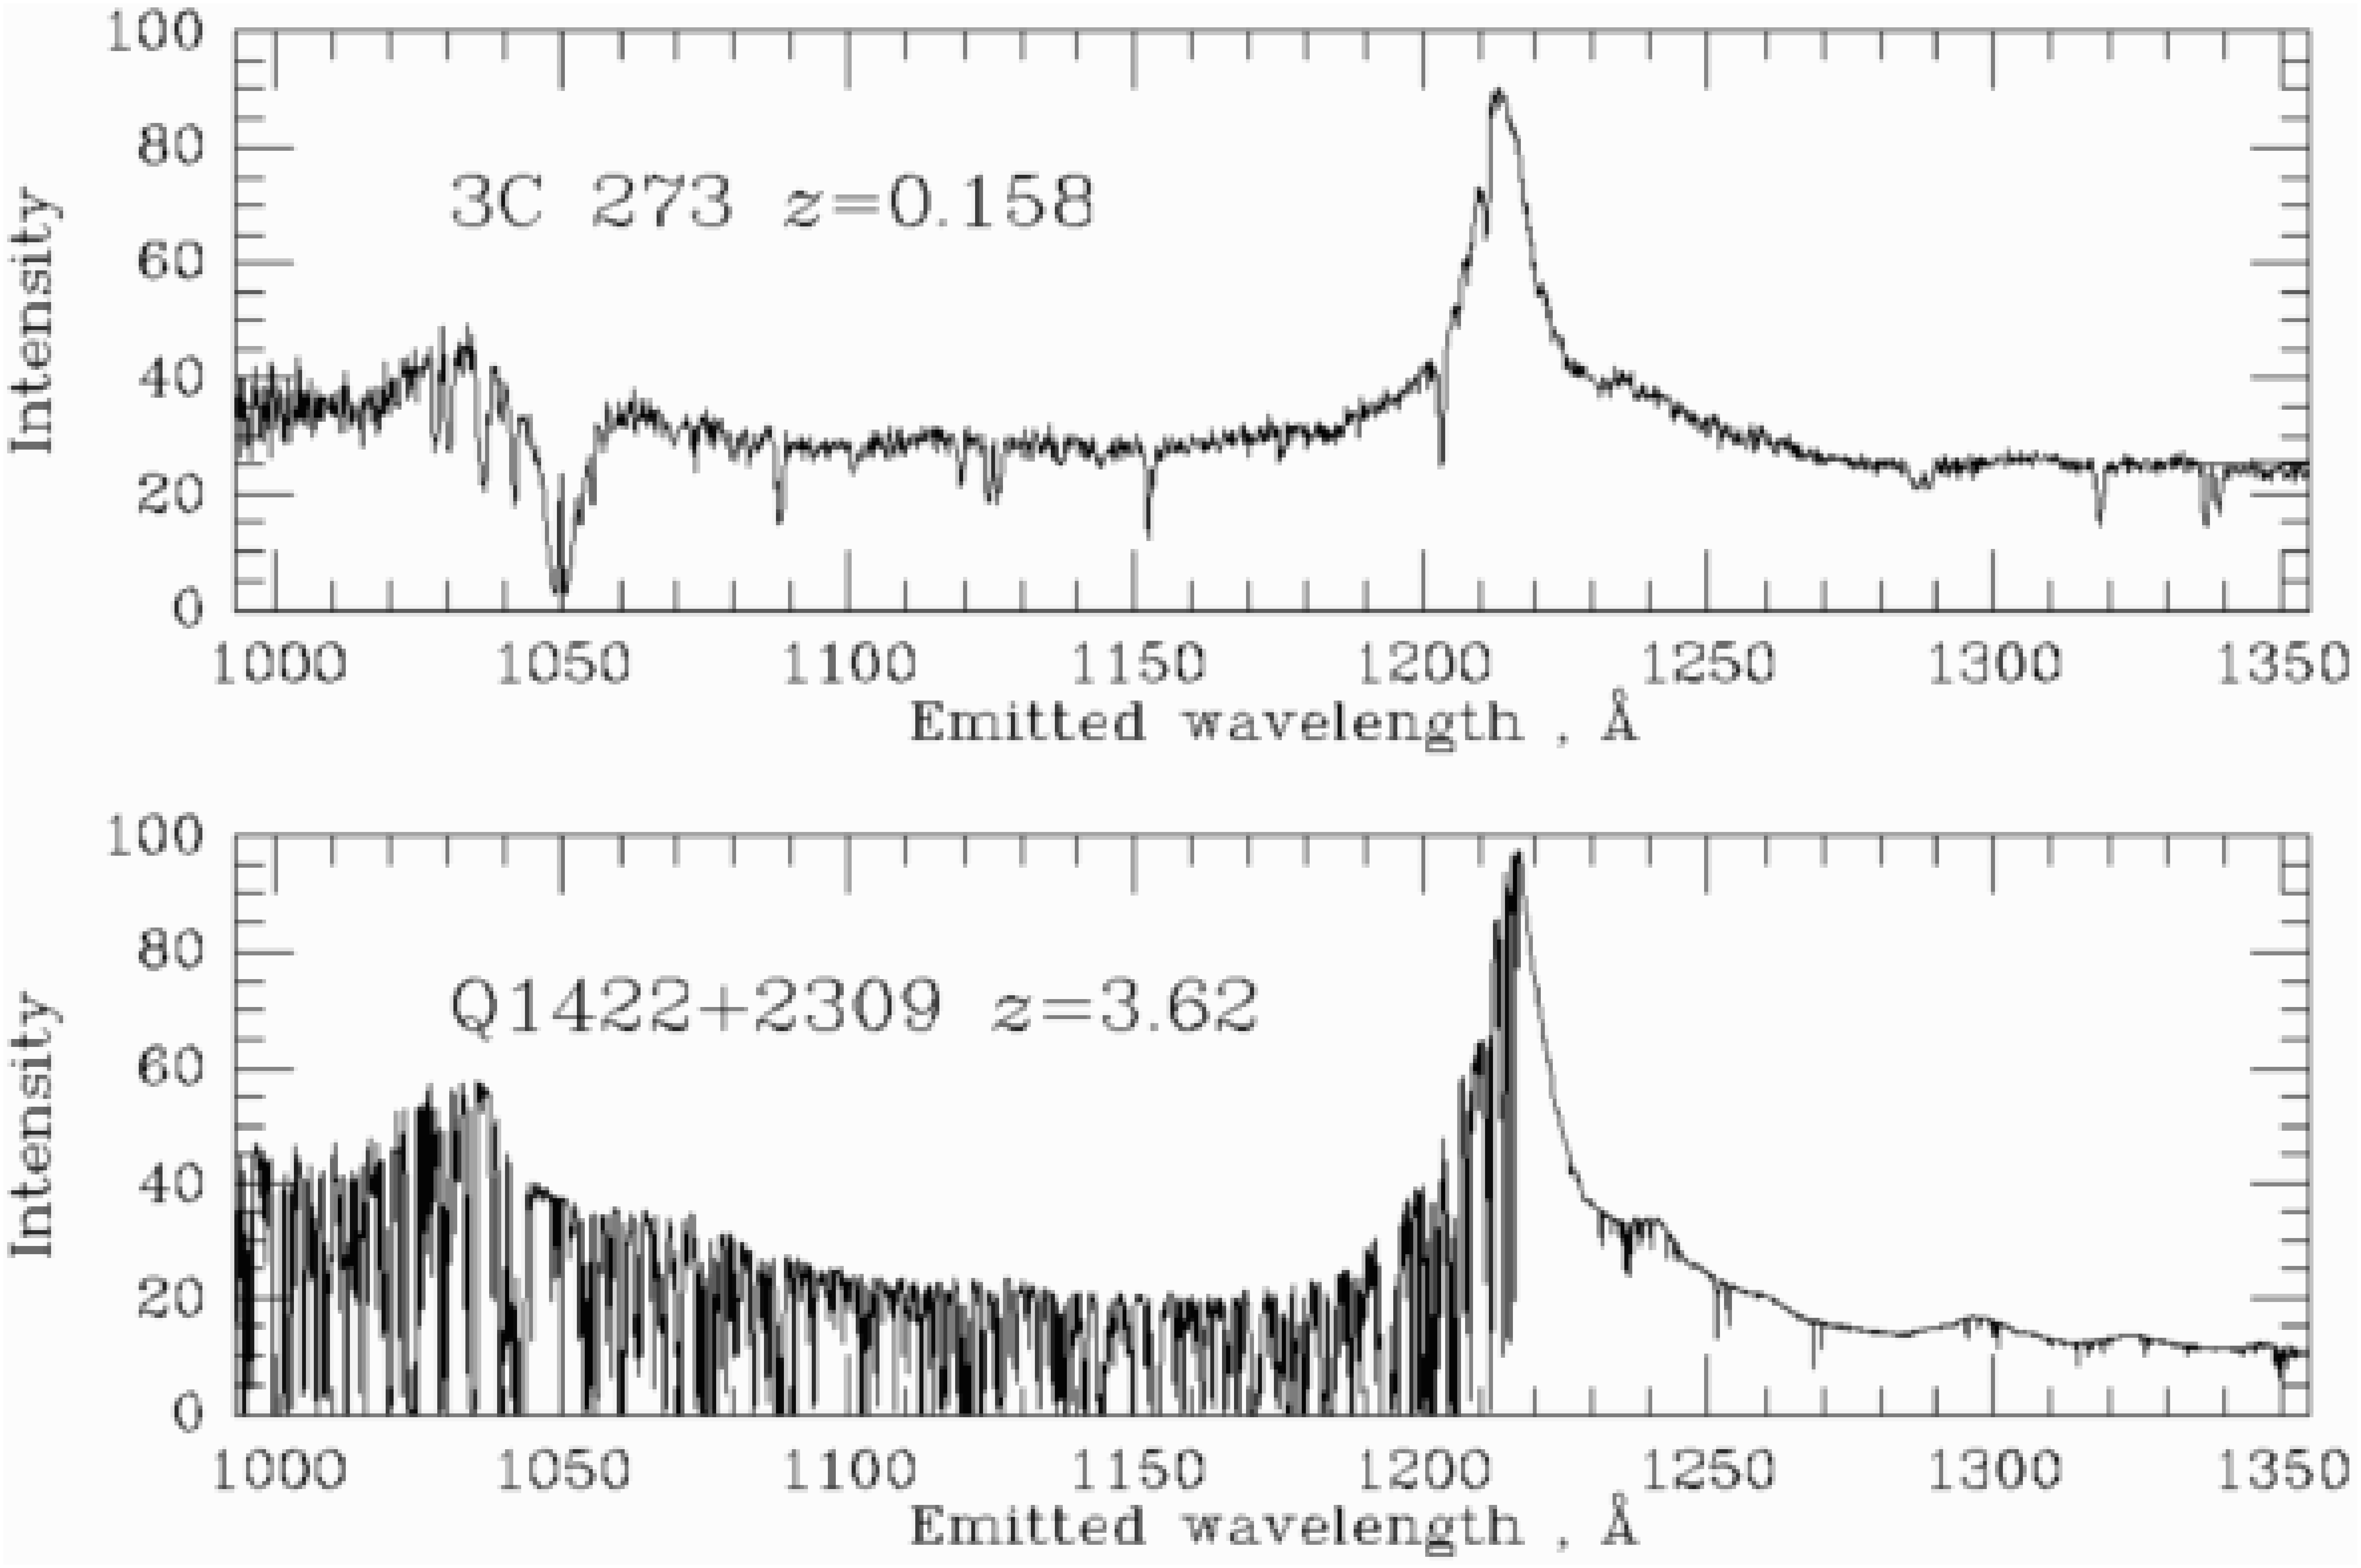
\includegraphics[width=12cm]{Lya-forest-60.eps}
  \caption{Flux as a function of rest-frame wavelength for a quasar at $z = 0.158$ (top) and $z = 3.62$ (bottom). The denser IGM at higher $z$ results in a dense ``forest" of absorption lines blueward of the rest-frame \lya\ line in the lower panel. (Image from {\tt http://www.astro.ucla.edu/})}
  \label{fig:LyaExample}
\end{figure}

At this point, the \lya\ forest should sound like a perfect tool: if we want to map the distribution of neutral hydrogen along the line of sight to a distant bright source, we can simply map each absorption line in the \lya\ forest to a parcel of neutral hydrogen. However, the story becomes complicated here due to the extremely large cross section for \lya\ absorption. Namely, the optical depth\nomenclature[Zp]{Optical Depth}{Optical depth, denoted by $\tau$, is a quantity that describes that likelihood for a photon to be absorbed, usually by a gas. The fraction of photons that will pass through the gas unabsorbed is $e^{-\tau}$.} for \lya\ absorption of a neutral hydrogen gas parcel obeys the relationship

\begin{align}
\tau_{\alpha} &\approx 3.3 \times 10^{4} \xhi (1 + \delta) \left[\dfrac{1+z}{6.5}\right]^{3/2}. \label{eq:tauGP}
\end{align}

Using this expression, we can calculate the minimum neutral fraction needed for a gas parcel at mean density to allow 1\% transmission at $z = 5.5$:

\begin{align}
.01 &= e^{-\tau_{\text{min}}} \implies \tau_{\text{min}} \approx 4.6\\
4.6 &\approx \tau_{\alpha} x_{\text{HI,min}} \\
\implies x_{\text{HI,min}} &\approx 0.00014.
\end{align}


This reveals the fly in the ointment here: even a gas parcel that is 99.9\% ionized will allow less than 1\% transmission at the redshifts of interest for reionization. This allows absorption features to be caused by highly-ionized gas that happens to be over-dense. Therefore, we can not simply map absorption lines in the \lya\ forest to regions of significantly-neutral hydrogen. In fact, the second example quasar we see in Figure \ref{fig:LyaExample} shows significant \lya\ absorption and is located at $z = 3.62$, \textit{much later than the end of reionization}. At this point, the reader may ask what utility does the \lya\ forest have at all? Well, an enormous amount. To name a very few applications outside of reionization, since \lya\ absorption can be caused by matter overdensities the \lya\ forest can be used to measure the matter power spectrum in the IGM which in turn can be used to measure the baryon acoustic oscillations (BAO), provide lower limits on the mass of the dark matter (\citealt{Viel:2013fqw}), and constrain dark energy. Additionally, absorption features due to damped \lya\ absorbers (DLAs) can be used to measure the primordial deuterium abundance as a test of big bang nucleosynthesis.\\
\textcolor{white}{suspense!}\\
\noindent But how to constrain the EoR?



\subsubsection{Evolution of $\tau_{\text{eff}}$}

% The Gunn-Peterson optical depth to \lya\ photons is \tau_{\text{GP}} = \dfrac{\pi e^2}{m_e c} f_{\alpha} \lambda_{\alpha} H^{-1}(z)n_{\text{HI}}

% Absorption is understood as being caused by the fluctuating Gunn-Peterson effect, low density regions in approximate thermal equilibrium between photoionization heating by the UV background and adiabatic cooling due to the Hubble expansion, rather than discrete \lya\ absorbers.

% By studying the evolution of the average transmitted flux or effective optical depth, one can trace the evolution in the 

% You probably want to re-read and refer to Lidz et al. that discuss that the evolution in the effective optical depth can be replicated by density fluctuations

Perhaps the most common analysis performed on high-redshift quasar spectra in the context of constraining the EoR is measurements of the effective Gunn-Peterson optical depth, defined as

\begin{align}
\langle F \rangle &\equiv e^{-\tau_{\text{eff}}}
\end{align}
where $\langle F \rangle$ is the averaged transmission fraction over a redshift bin. Under the assumption of ionization equilibrium, where the rate that neutral hydrogen atoms are ionized is equal to the rate that they recombine, the effective optical depth encodes important information about the state of the IGM. In order to see this, we can take a few steps to express the optical depth in terms of the properties of the IGM.\footnote{The following discussion will borrow heavily from \cite{FaucherGiguere:2007jc} and \cite{fan2002evolution}.} First, the Gunn-Peterson optical depth can be expressed as

\begin{align}
\tau_{\text{GP}} &= \dfrac{\pi e^{2}}{m_{e} c} f_{\alpha}\lambda_{\alpha} \dfrac{n_{\text{HI}}}{H(z)}, \label{eq:tauGP}
\end{align}

where $H(z)$ is the Hubble parameter at redshift $z$. All of these quantities are known with the exception of the number density of neutral hydrogen atoms, $n_{\text{HI}}$. To find this, we first utilize the statement of ionization equilibrium:

\begin{align}
\Gamma_{\text{HI}} n_{\text{HI}} &= R(T)n_{e}n_{\text{HII}} \label{eq:IonEquilibrium} \\
n_{\text{HI}} &= \dfrac{R(T) n_{e} n_{\text{HII}}}{\Gamma_{\text{HI}}} \label{eq:nH}\\
x_{\text{HI}} &= \dfrac{R(T)n_e}{\Gamma_{\text{HI}}} \label{eq:xHI}
\end{align}

where $\Gamma_{\text{HI}}$ is the photoionization rate due to the ionizing sources, $n_{\text{HI}}$ is the number density of neutral hydrogen atoms, $n_{e}$ is the number density of free electrons, $n_{\text{HII}}$ is the number density of ionized hydrogen atoms (protons), and $x_{\text{HI}}$ is the hydrogen neutral fraction. Clearly, the left-hand side of Eq. \ref{eq:IonEquilibrium} represents the rate of photoionizations per volume and the right hand side represents the rate of hydrogen recombinations per volume. Under the assumption of ionization equilibrium, it is true that $n_{\text{HII}} \approx n_{\text{HI}} + n_{\text{HII}} = n_{\text{H}}$ and 

\begin{align}
\bar{n}_{\text{H}} &= \frac{\rho_{c}(z)\Omega_{b}(z)X_{\text{H}}}{m_p} = \dfrac{3H^{2}(z)}{8\pi G} \dfrac{\Omega_{b}(z) X_{\text{H}}}{m_{p}} \\
&= \dfrac{3H_{0}^{2}\Omega_{b,0}}{8\pi G} \dfrac{X_{\text{H}}}{m_p}(1+z)^{3}\\
n_{\text{H}} &= (1+\delta) \bar{n}_{\text{H}}. \label{eq:ntot}
\end{align}

In this expression, $\rho_c$ is the critical density for a flat Universe, $\Omega_{b}$ is the baryon density in units of the critical density, $X_{\text{H}}$ is the fraction of baryonic mass in the form of hydrogen, $m_{p}$ is the mass of the proton which is effectively equal to the mass of the hydrogen atom, and $\delta = (\rho-\bar{\rho})/\bar{\rho}$ is the local overdensity in units of the cosmic mean. A subscript of ``0" denotes that these are present-day values and $\bar{n}_{\text{H}}$ denotes the average of $n_{\text{H}}$. Thus, as we expect, this expression is essentially equal to the mass density of hydrogen atoms in the Universe divided by the mass per atom.\footnote{It may be interesting to note that this value corresponds to 4 hydrogen atoms per cubic meter today and roughly $\sim$1100 hydrogen atoms per cubic meter at $z = 5.5$.}  The expression for the electron number density should be the same, since each ionized hydrogen atom releases one free electron. However, it is probably the case that helium is singly ionized along with hydrogen, so the number density will increase according to:

\begin{align}
\bar{n}_e &= \bar{n}_{\text{H}} + \bar{n}_{\text{He}} = \dfrac{3H^2}{8\pi G}\left( \dfrac{X_{\text{H}}}{m_{p}} + \dfrac{(1 - X_{\text{H}})}{4m_{p}} \right) \\
&\approx 1.08 \bar{n}_{\text{H}}. 
\end{align}

However, for simplicity, let us approximate $n_{\text{tot}} \equiv n_{e} \approx n_{\text{H}}$. The quantity $R(T)$ in Eq. \ref{eq:IonEquilibrium} is the recombination rate, which is equal to

\begin{align}
R(T) &\approx 4.2 \times 10^{-13}\left( \dfrac{T}{10^{4} K}\right)^{-0.7} \text{cm}^{3}\sec^{-1}. \label{eq:RecombinationRate}
\end{align}

For $\delta \lesssim 5$, \cite{Hui1997} showed that the temperature and density follow the relationship

\begin{align}
T &\approx T_{0}(1+\delta)^{\gamma - 1} \label{eq:Trelation}
\end{align}

where $\delta \equiv (\rho - \bar{\rho})/\bar{\rho}$ is the baryon overdensity in units of the cosmic mean density, $T_0$ is the temperature of a parcel of gas at mean density, and $\gamma$ is the slope of the temperature-density relation. For compactness, let's define $R_{4} \equiv R(T=10^{4}K)$. At this point, we are ready to combine Eq. \ref{eq:Trelation}, \ref{eq:RecombinationRate}, \ref{eq:ntot}, \ref{eq:nH}, and \ref{eq:tauGP} to get an expression for $\tau_{\text{GP}}$:

\begin{align}
\tau_{\text{GP}} &= \dfrac{\pi e^2}{m_e c}\dfrac{f_{\alpha}\lambda_{\alpha}}{H(z)} \dfrac{R_{4}(1+\delta)^{-0.7(\gamma - 1)}\bar{n}_{\text{tot}}^{2}(z)(1+\delta)^2}{\Gamma_{\text{HI}}}\\
&= \dfrac{\pi e^2}{m_e c}\dfrac{f_{\alpha}\lambda_{\alpha}}{H(z)} \dfrac{R_4 \bar{n}_{\text{tot}}^{2}(z)}{\Gamma_{\text{HI}}} (1+\delta)^{2-0.7(\gamma-1)}. \label{eq:tauGPfinal}
\end{align}

Finally, we have an expression for the \lya\ optical depth in terms of several properties of the IGM. The primary unknown in the above expression is the photoionization rate, which is a very complicated parameter which depends on the number, intensity, spectrum, and proximity of ionizing sources among other things. A common assumption in these types of analyses is that the photoionization rate is approximately spatially uniform. This seems like a plausible assumption in a post-reionization Universe, when any given gas parcel can receive ionizing radiation from hundreds of sources. On the other hand, early in reionization, the Universe is opaque to ionizing radiation and gas parcels tend to only see sources within their own ionized regions. Regardless, with this approximation, the observed mean transmission in a region of the spectrum is akin to an average of Eq. \ref{eq:tauGPfinal} over the density field:

\begin{align}
\left\langle F \right\rangle &= \int \dd \delta\ e^{-\tau(\delta)} P(\delta) \equiv e^{-\tau_{\text{eff}}}.
\end{align}


 As such, an intriguing question is, if you have a model for the probability distribution of the underlying density field, what (uniform) value of $\Gamma_{\text{HI}}$ will yield a value for $\left\langle F \right\rangle$ that is consistent with observations? This question has received a lot of attention ({\bf cites}) and has led to many measurements of the photoionization rate. With estimates of the photoionization rate in hand, we can utilize Eq. \ref{eq:xHI} in order to obtain measurements of the IGM neutral fraction in each redshift bin in order to gauge the progress of the EoR. Results for measurements of $\Gamma_{\text{HI}}$ and $\axhi$ via this method, performed by \cite{Fan2006a}, are shown in Figure \ref{fig:tauEffResults}. This figure demonstrates that, using $\tau_{\text{eff}}$ and the assumption of ionization equilibrium, estimates of the neutral fraction are exceedingly small for $z \lesssim 6$. This argument has played a large part in forming the common knowledge that reionization has ended by $z = 6$. 

\begin{figure}[h]
  \centering
  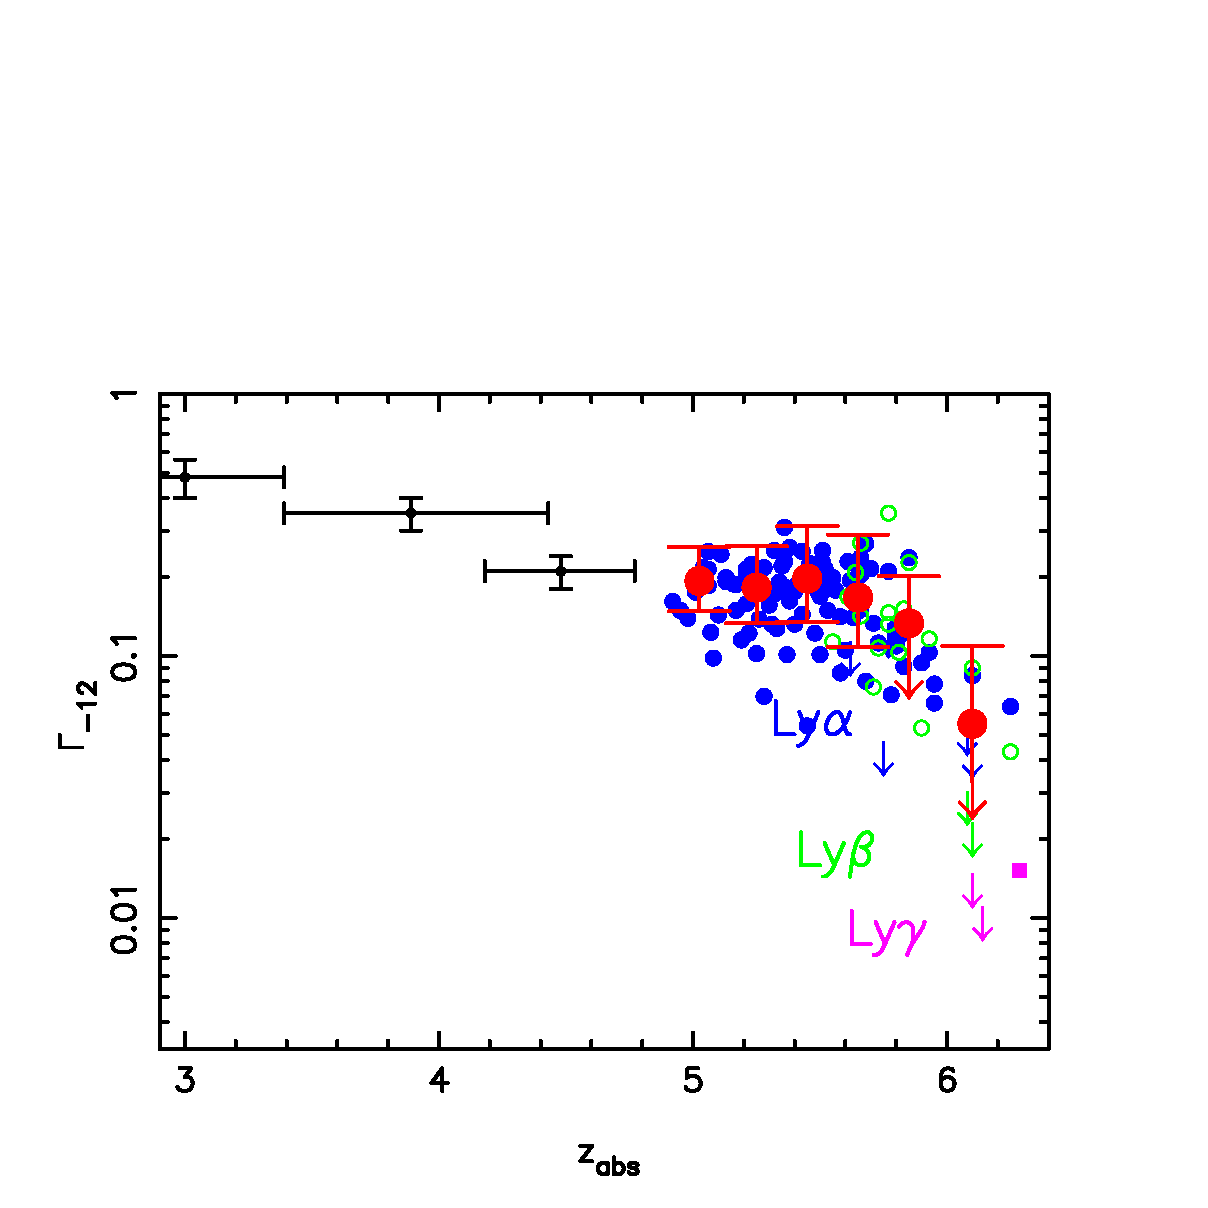
\includegraphics[width=8cm]{Fan.gamma.eps}
  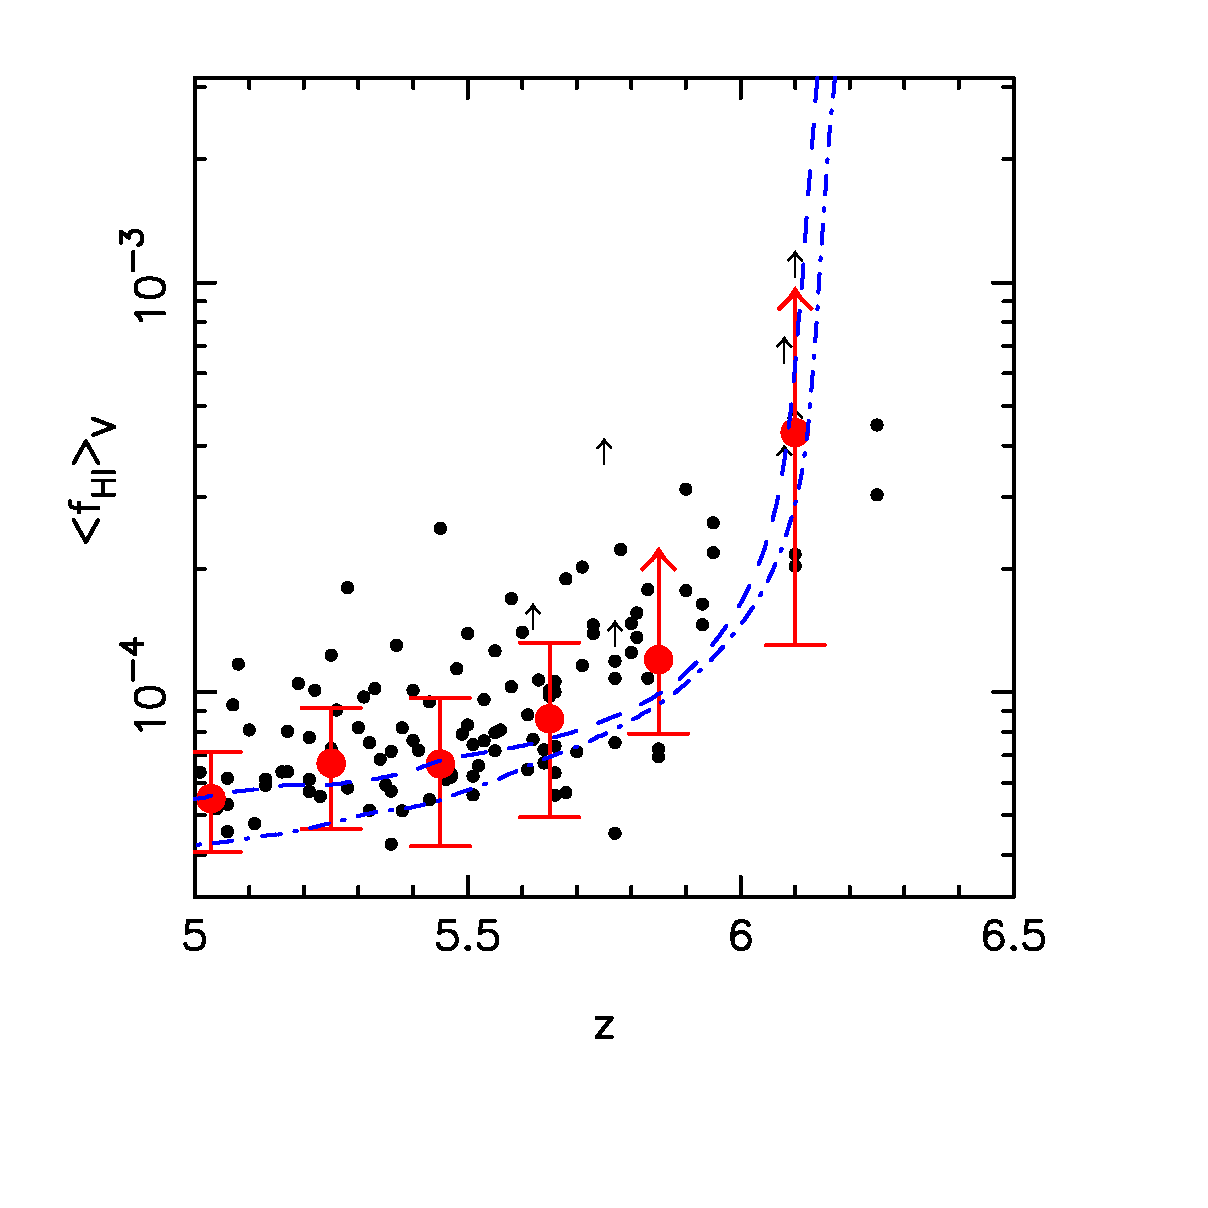
\includegraphics[width=8cm]{Fan.fHv.eps}
  \caption{Measurements of $\Gamma_{\text{HI}}$ (top) and $\axhi$ from \cite{Fan2006a} (bottom).}
  \label{fig:tauEffResults}
\end{figure}


Despite the widespread analysis of $\tau_{\text{eff}}$ in constraining the end of reionization, the interpretation of $\tau_{\text{eff}}$ is quite complicated.\footnote{For a more thorough discussion of controversial aspects of these constraints, see the intro for \cite{McGreer:2011dm}.} First, accepting the assumption of the IGM being in ionization equilibrium with a uniform $\Gamma_{\text{HI}}$ is tantamount to assuming that reionization has ended. Specifically, as discussed in \S \ref{sec:CosmicContext}, reionization is likely a highly inhomogeneous process with ionized bubbles forming around the brightest sources, growing, and eventually overlapping. During the period prior to complete overlap, regions of neutral hydrogen will be shielded from the ionizing radiation while ionized bubbles will experience a very large $\Gamma_{\text{HI}}$. This is not reflected in Eq. \ref{eq:IonEquilibrium} and so we expect conclusions derived from this method to be unreliable when we begin to push up against the end of reionization. Additionally, interpretation of the level of flux in quasar spectra in the context of reionization is further complicated by the fact that quasars likely reside in very atypical parts of the Universe. Specifically, \cite{Lidz:2007mz} show that it is likely that many quasar lines of sight will pass through mostly ionized gas even up to neutral fractions of $\axhi \sim 0.5$. 

%\subsubsection{Dark Gap Sizes}
%
%Yeah, so the main point we want to (briefly) drive home here is that previous constraints on $\axhi$ from the use of dark gap statistics probably assumed a uniform $\Gamma_{\text{HI}}$, which is equivalent to assuming reionization has already ended anyway. 
%
%Fan says imperfect sky subtraction in regions with strong OH lines can cause significant residuals resulting in an \textit{underestimate} in the dark gap size. Although, it seems like they don't allow any room for noise fluctuations in what they constitute a dark gap???


\subsubsection{Dark Pixel Covering Fraction}

As demonstrated in the previous section, interpreting measurements of the effective optical depth in the context of reionization is complicated and often relies on suspicious . However, an alternative approach is to consider what constraints can be made without resorting to model-dependent assumptions. In this regard, an important method in estimating $\axhi$ from high-redshift quasar observations is the dark pixel covering fraction. This approach is rooted in the fact that neutral parcels of gas are certain to result in saturated absorption in quasar spectra due to their optical depths being $\tau_{\text{HI}} \gtrsim 10^4$ (Eq. \ref{eq:tauGP}). Therefore, a reliable upper bound on the neutral fraction at a given redshift can be estimated by the fraction of pixels in quasar spectra that are completely absorbed at that redshift. 

An obvious drawback of this method is that, at $z \sim 6$, overdense yet ionized regions can very well result in saturated absorption as well and significantly increase the upper bound on the neutral fraction. One approach to combat this effect is to incorporate the \lyb\ forest into the analysis. The optical depth for Lyman-series transitions scales as $f\lambda$, where $f$ is the oscillator strength of the transition and $\lambda$ is the corresponding wavelength. Therefore, the analogous expression of Eq. \ref{eq:tauGP} for \lyb\ is:

%Useful quantities:                                                                                                   
% Oscillator Strengths                                                                                                
% f_21 = 0.4162 (1s-2p)  lambda_21 = 1215.67 AA                                                                       
% f_31 = 0.0791 (1s-3p)  lambda_31 = 1025.72 AA                                                                       
% f_32 = 0.4349 (2s-3p)  lambda_32 = 6562.74 AA 
\begin{align}
\tau_{\beta} &= \tau_{\alpha} \times \dfrac{f_{\beta}\lambda_{\beta}}{f_{\alpha}\lambda_{\alpha}} \approx 5.3 \times 10^{3} \xhi (1 + \delta) \left[\dfrac{1+z}{6.5}\right]^{3/2}. \label{eq:tauGPB}
\end{align}

where $f_{\alpha} = 0.4162$, $\lambda_{\alpha} = 1216 \AA$, $f_{\beta} = 0.0791$, and $\lambda_{\beta} = 1026\AA$. From this expression, we can see that a mean-density parcel of neutral gas should cause saturated absorption in both the \lya\ and \lyb\ transitions. Meanwhile, ionized overdense regions are less likely to cause saturated absorption as their optical depth in \lyb\ is reduced by a factor of $f_{\beta}\lambda_{\beta}/f_{\alpha}\lambda_{\alpha} \approx 1/6$. Therefore, limits from the dark-pixel covering fraction may be improved by requiring simultaneous absorption in both \lya\ and \lyb\ as part of the definition of a dark pixel. Additionally, the \lyb\ dark pixel covering fraction on its own is a viable tool for establishing an upper bound on the neutral fraction, although foreground \lya\ absorption may undo some of the gains from the lower $\tau_{\beta}$ value.

This procedure faces several complications when actually carried out, however. First, quasar observations are subject to the noise from the night sky which effectively adds mean-zero random noise to the spectra. The addition of this random noise can result in spurious transmission in pixels that otherwise would have been completely absorbed. Therefore, to measure the dark pixel fraction in quasar spectra, one first needs to create a suitable definition of what classifies as a ``dark" pixel. One approach here is to define dark pixels as having transmission below some threshold defined in terms of the noisy standard deviation, $\sigma_{\text{N}}$. This presents us with a tradeoff, however, since larger thresholds will reduce the number of neutral pixels we miss but also increase the number of ionized pixels that get incorporated into the dark pixel population.

A second complication is that, since pixels have a finite width, their transmission values effectively represent an average of the transmission over some region in the spectra. If the pixel width is large enough, then it is possible for a pixel to have non-zero transmission despite corresponding to a physical region that contains significantly-neutral gas. For example, if the physical region in space associated with the pixel is 80\% composed of completely-neutral gas and 20\% composed of completely ionized gas which allows full transmission, then the transmission of that pixel will be 20\% and will likely not qualify as a ``dark pixel" despite containing neutral gas. Thus, even in a measurement as seemingly-simple as the dark-pixel covering fraction, these details must be kept in mind when interpreting results.

Regardless, \cite{McGreer:2011dm} and \cite{McGreer:2014qwa} apply the dark-pixel covering fraction approach to 22 high-redshift quasar spectra to produce the constraints on $\axhi$ shown in Figure \ref{fig:McGreer}. Dimly-colored points correspond to \cite{McGreer:2011dm} while bold-colored points correspond to \cite{McGreer:2014qwa}. The main conclusion here is that model-independent constraints have a hard time conclusively confirming the common knowledge that reionization has ended by $z \sim 6$.\footnote{The authors here do go on to focus on a high-resolution subset of their quasar observations in order to argue in favor of an end to the EoR by $z \sim 6$. However, the precise interpretation of the spectra is complex, as discussed herein.} 

\begin{figure}[h]
  \centering
  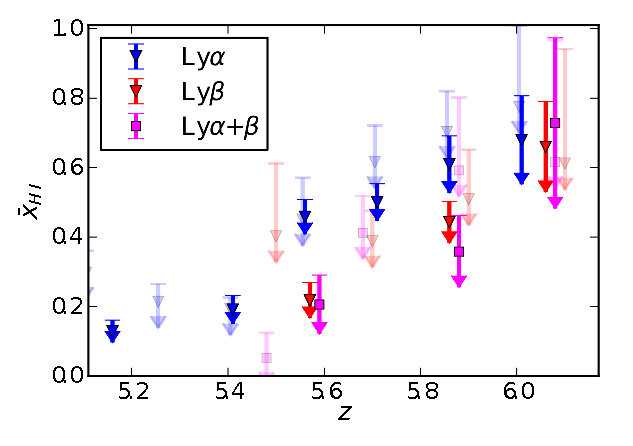
\includegraphics[width=8cm]{xhi_newdata.eps}
  \caption{Current limits on $\axhi$ derived from the dark-pixel covering fraction in \cite{McGreer:2014qwa}. Lightly-shaded points are older limits obtained in \cite{McGreer:2011dm}.}
  \label{fig:McGreer}
\end{figure}



\subsubsection{Damping Wing Redward of \lya}\label{sec:IntroDampingWing}

Much of the difficulties in using the \lya\ forest to constrain the timing of the EoR can be boiled down to the following problem: interpreting \lya\ absorption in high-redshift quasar spectra is difficult because both neutral and ionized gas can result in saturated absorption. Therefore, it is worth asking if there are any ways to break this degeneracy in \lya\ absorption in order to determine which absorption is likely due to neutral hydrogen. One potential approach toward this goal, which has received much attention (\cite{Chornock:2013una}, \cite{Chornock:2014fva}, \cite{Mortlock2011}, \cite{Bolton:2011vb}), is looking for the hydrogen damping wing redward of the \lya\ line. 


To understand this approach, let us first understand what the hydrogen damping wing is. For many applications, it is suitable to consider an atom's ability to absorb radiation as a series of delta functions in frequency: when incident radiation has a frequency exactly coinciding with the energy of the transition, then there is a non-zero probability for absorption and zero probability otherwise. In reality, the probability of absorbing a photon of a given frequency, e.g., the line profile, is a continuous distribution which, while small for frequencies $\nu \neq \nu_{0}$, is non-zero. 


The intrinsic line profile for the \lya\ transition in the hydrogen atom can be seen as arising from the time/energy uncertainty principle, $\Delta E \cdot \Delta t \gtrsim \hbar$. Specifically, the finite lifetime of the $n = 2$ excited state implies the existence of a range of energies that can excite, or result from, the transition. The distribution of this range of energies follows a Lorentzian distribution \gloss{Lorentzian Distribution}{Probability distribution for the ratio of two standard-normal-distributed variables. This distribution also describes the intrinsic line profile for absorption lines.}:

\begin{align}
\phi(\nu) &= \frac{1}{\pi} \dfrac{\Gamma/4\pi^{2}}{(\nu - \nu_{0})^{2} + (\Gamma/4\pi)^2}
\end{align}

with the corresponding absorption cross section

\begin{align}
\sigma_{\alpha}(\nu) &= \dfrac{\pi e^2}{m_{e}c} f_{\alpha} \phi(\nu). \label{eq:IntroLineProfile}
\end{align}

The ``damping wing" refers to the $\sigma \sim 1/(\nu-\nu_{0})^{2}$ behavior far from line center. This can be used to break the degeneracy between HII absorption and HI absorption because the optical depth is so much smaller in the damping wing that, without significantly-neutral gas (optical depth scales with neutral fraction), the optical depth at such frequency separations will not be sufficient to cause absorption. Furthermore, the damping wing has a distinct shape which can be fit for in order to infer the properties of the neutral gas which sources it. 


While the damping wing from an isolated neutral region in a sea of fully-ionized, $\tau = 0$ hydrogen would stand out like a sore thumb, in reality absorption from the surrounding dense, yet ionized, gas will punctuate the damping wing with additional absorption features and will make it harder to detect. This makes the prospect of looking for isolated damping wings in typical regions in quasar spectra unappealing. However, photons emitted slightly \textit{redward} of \lya\ cannot be absorbed by dense ionized gas since ionized gas has a negligible optical depth for $\nu \neq \nu_{\alpha}$. Neutral hydrogen, on the other hand, \textit{will} allow absorption to take place redward of \lya\ due to the significant optical depth in the damping wing. Because of this, searches for the damping wing slightly redward of the \lya\ line will be able to avoid nuisance absorption from neighboring ionized gas.


We show the most well-known example of a potential damping-wing detection in Figure \ref{fig:Mortlock}, taken from \cite{Mortlock2011}. This shows a region of the transmission spectrum for a quasar at redshift $z = 7.085$ (ULAS J1120+0641). The fractional transmission nearby the \lya\ line exhibits a gradual recovery from almost complete absorption at $\lambda < \lambda_{\alpha}$ to almost complete transmission at $\lambda > \lambda_{\alpha}$, occurring over a wavelength interval consistent with a hydrogen damping wing. The curves in blue show models for damping wing absorption associated with an IGM with neutral fraction $\axhi = 0.1$ (top), 0.5 (middle), and 1 (bottom) with a sharp ionization front at a distance of 2.2Mpc from the quasar. In green, a model for the absorption profile of a Damped \lya\ Absorber (DLA) with column density $N_{\text{HI}} = 4\times10^{20}\text{cm}^{-2}$ located 2.6 Mpc from the quasar is shown. Thus, the transmission profile appears consistent with both a significantly-neutral ($\axhi > 0.1$) IGM or a proximate DLA. However, \cite{Simcoe} perform a search for metal lines, which typically accompany DLA absorption, and find that the gas is extremely metal-poor. This bolsters the claim that the damping-wing absorption seen in this example is, in fact, due to diffuse neutral hydrogen in the IGM. 


\begin{figure}[h]
  \centering
  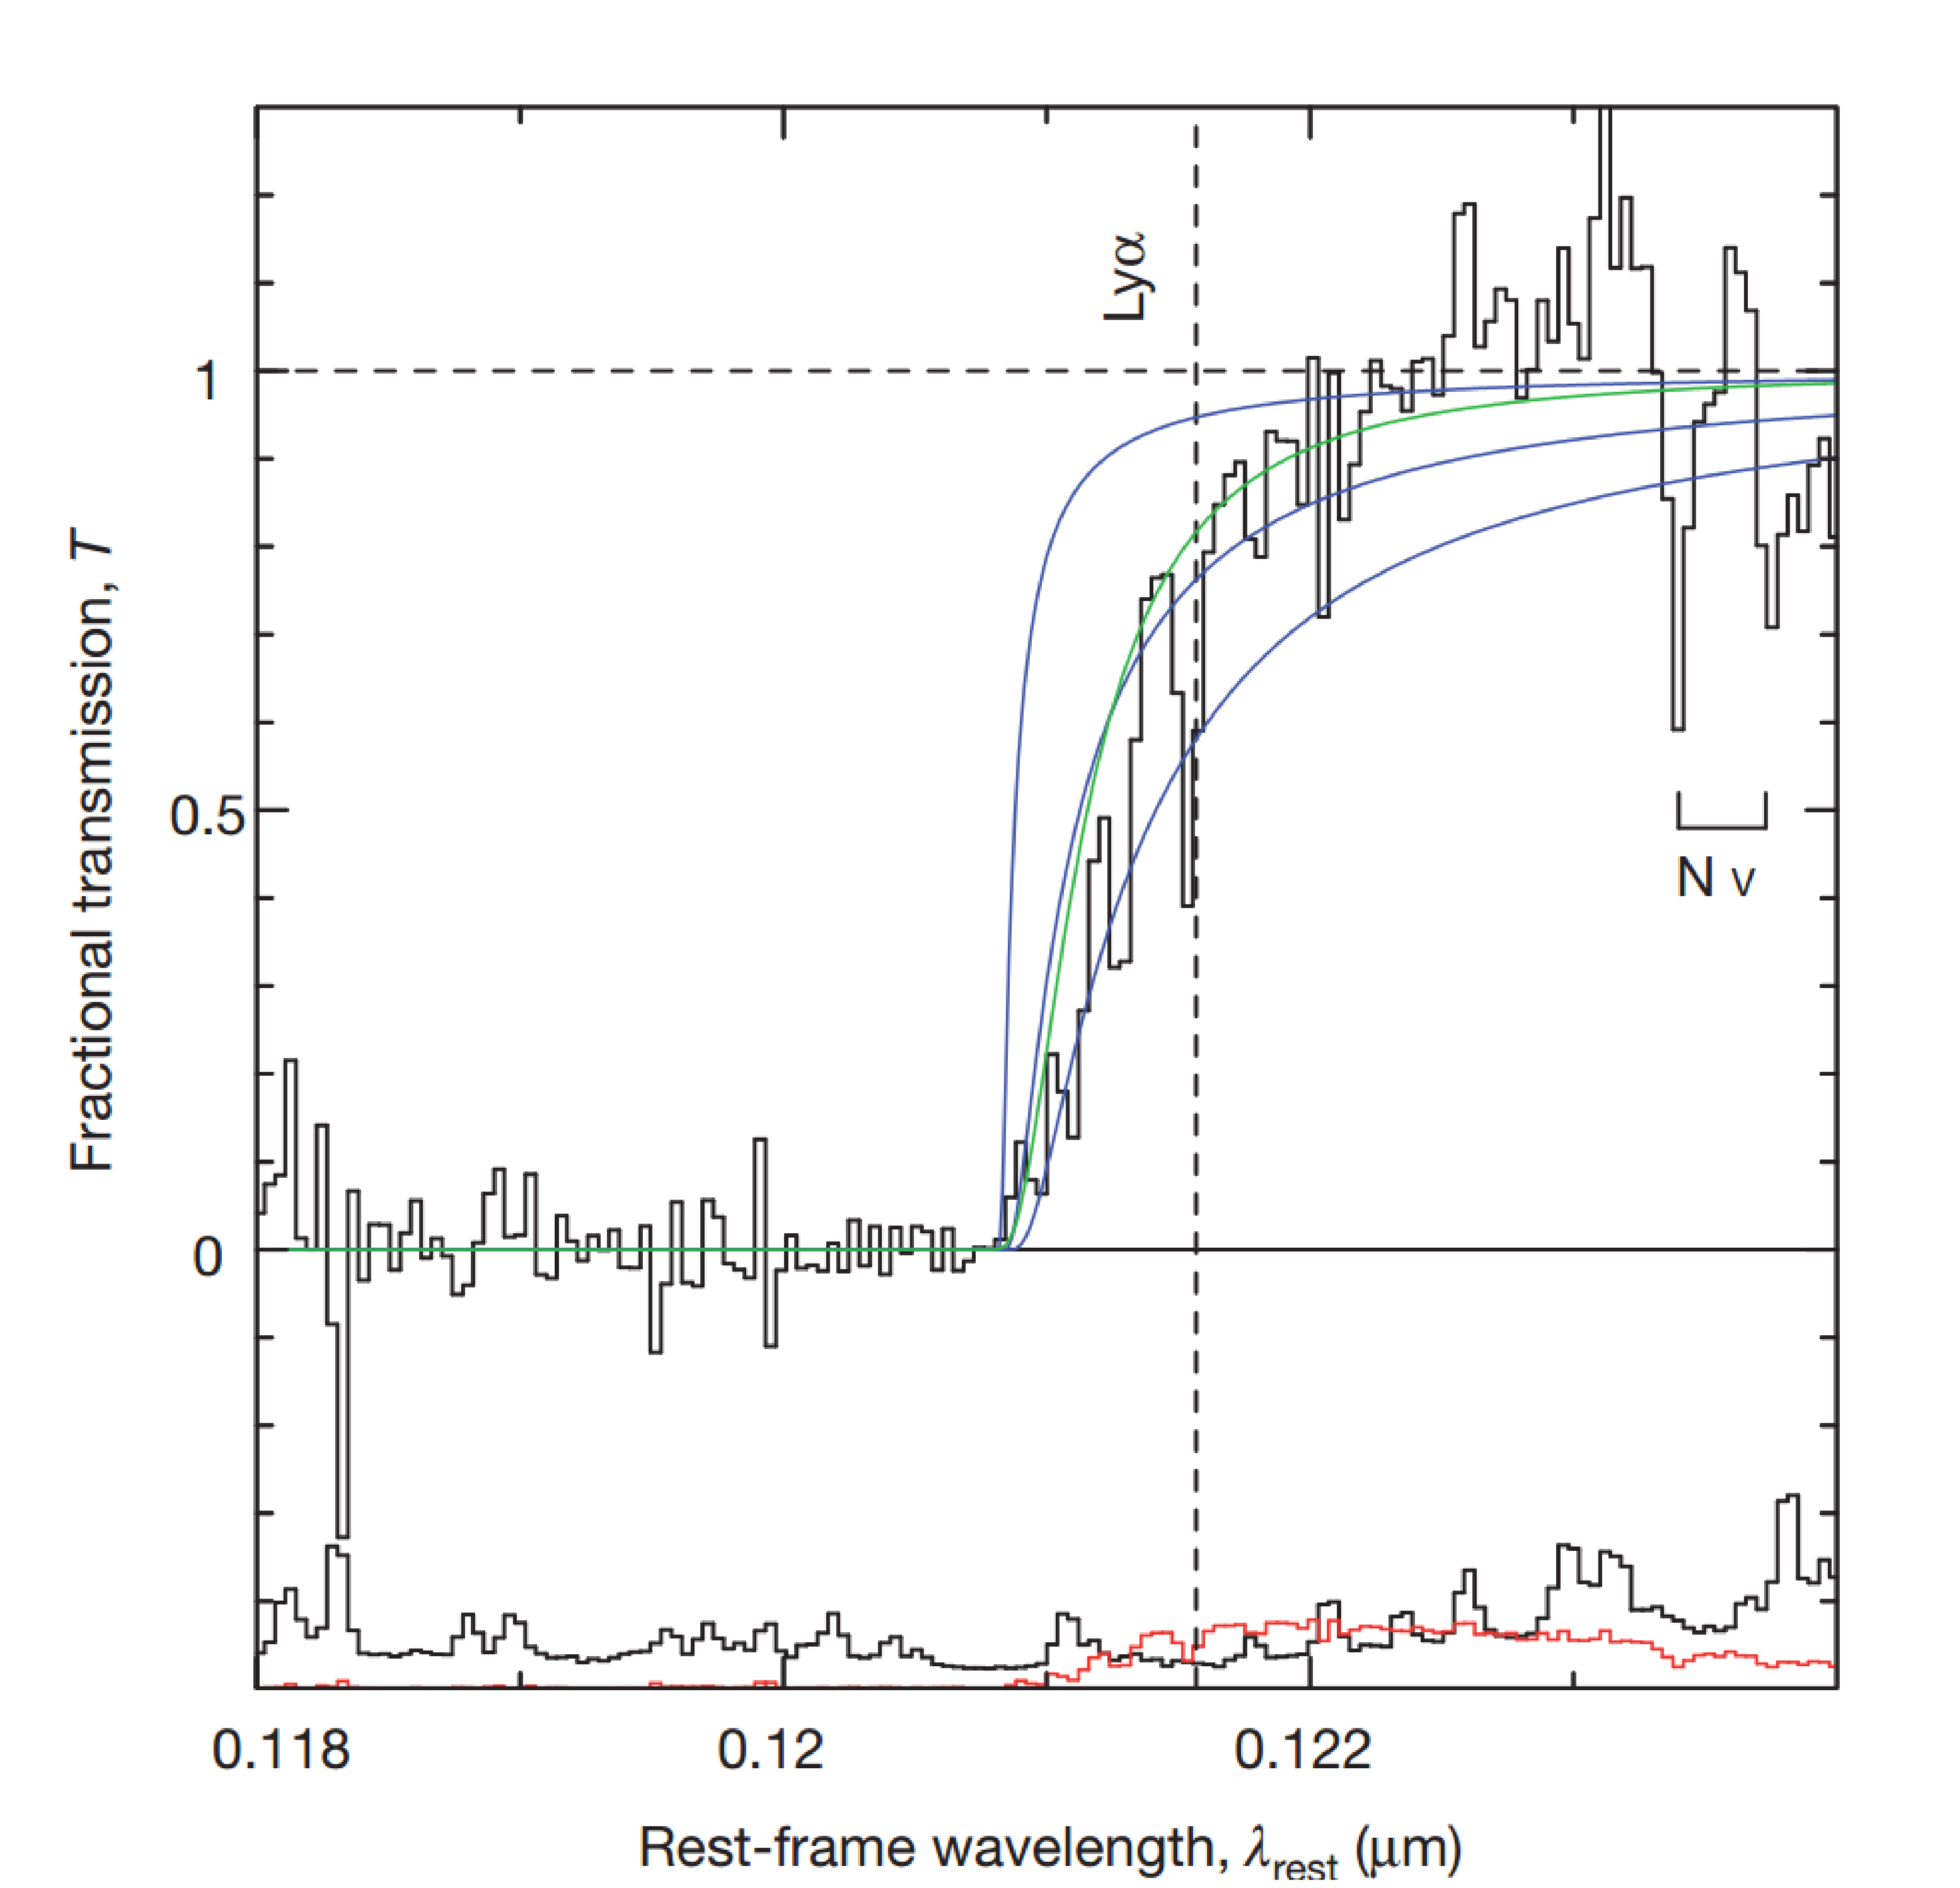
\includegraphics[width=8cm]{z7p085_DampingWing.eps}
  \caption{Quasar ULAS J1120+0641 identified at redshift $z = 7.085$ along with several fits for the damping wing.}
  \label{fig:Mortlock}
\end{figure}


Other searches for damping-wing absorption redward of \lya\ have been carried out on, for example, GRB 130606A (\citealt{Chornock:2013una}) and GRB 140515A (\citealt{Chornock:2014fva}). These authors looked for the damping wing in the spectra of GRB afterglows at redshift $z = 5.913$ and $z = 6.33$, respectively. A non-detection in the spectra of the $z = 5.913$ GRB allowed the authors to place a $2\sigma$ limit on the nearby IGM neutral fraction of $\axhi < 0.11$. Similarly, no strong evidence of a damping wing was found in the spectrum of GRB140515A, shown in Figure \ref{fig:GRB140515A}. The right-hand panel shows the transmission fraction nearby the \lya\ transition, which is equally-well fit by pure host absorption (blue, $N_{\text{HI}} = 10^{18.62}\text{cm}^{-2}$), pure IGM absorption from gas at $6.0 \leq z \leq 6.328$ with $\axhi = 0.056$ (red), and a hybrid model with a host absorber lying within an ionized bubble with $R = 10$ comoving Mpc met by an IGM with $\axhi = 0.12$ (green). As such, they argue against a significantly-neutral IGM at this redshift.  

\begin{figure}[h]
  \centering
  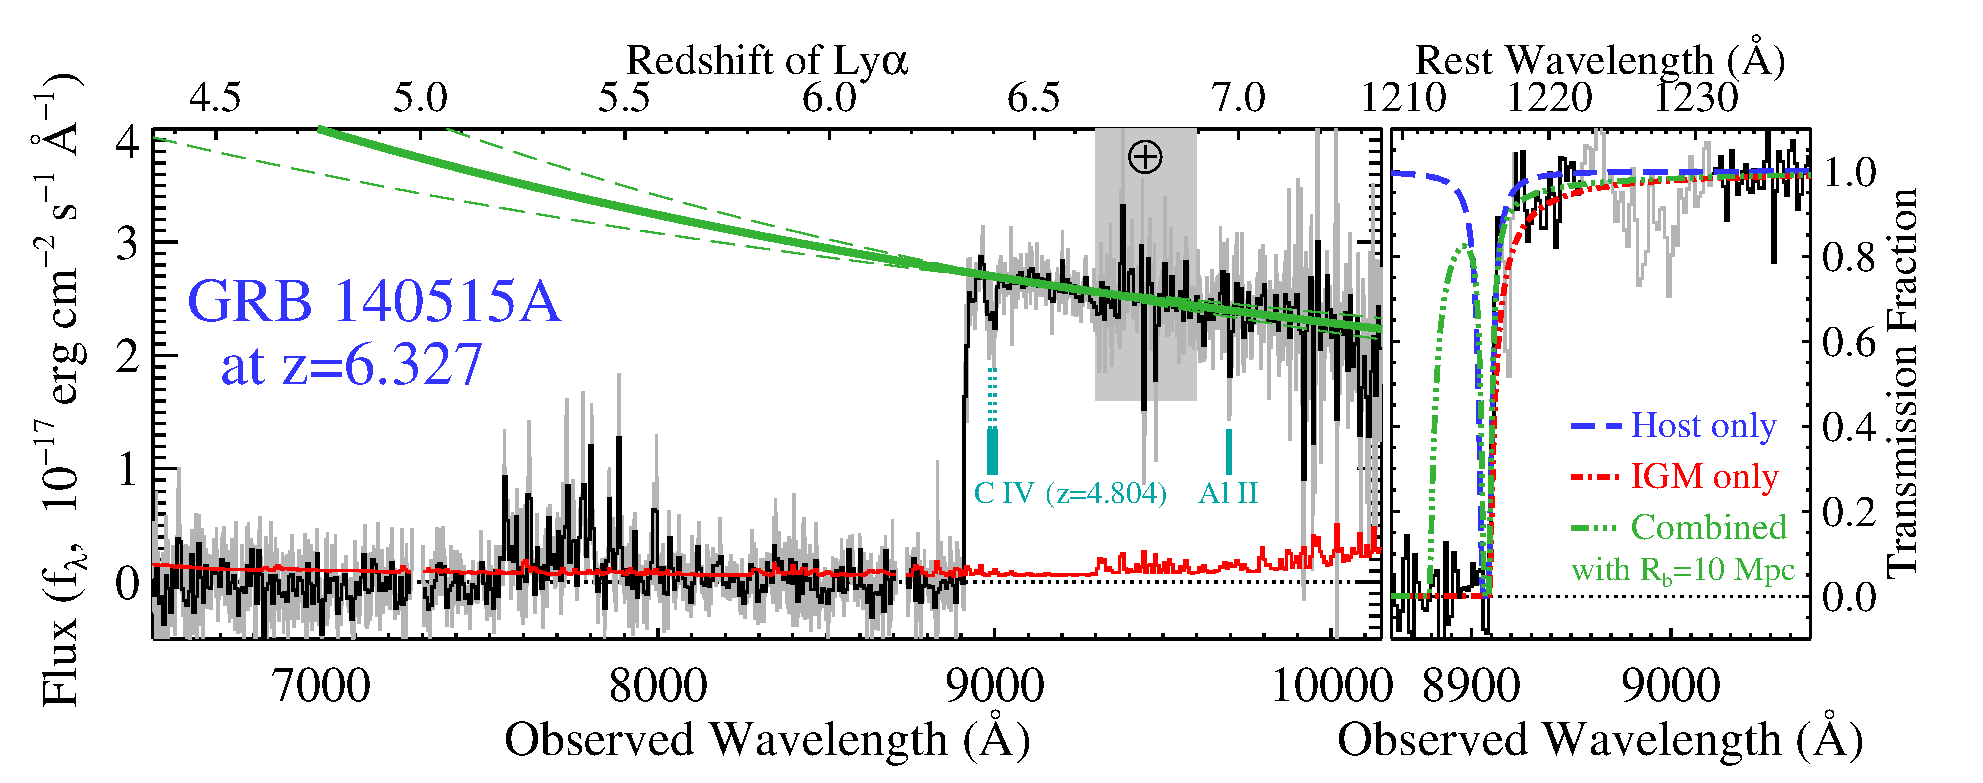
\includegraphics[width=14cm]{GRB140515A.eps}
  \caption{Spectrum of GRB140515A, a gamma-ray burst located at $z = 6.33$. The right-hand panel overlays damping wing models from a host absorber (blue), a pure IGM model with $\axhi = 0.056$ (red), and a combination model (green). The authors argue that, while each curve provides an equally-good fit to the data, the sharp rise in transmission shown is inconsistent with a significantly-neutral IGM. }
  \label{fig:GRB140515A}
\end{figure}


It is worth pointing out, however, that the method of searching for the damping wing redward of \lya\ is not without drawbacks. First, detecting the damping wing redward of \lya\ relies on your ability to understand what the quasar flux \textit{would have} been in the absence of the absorbing gas nearby the \lya\ line (this unabsorbed flux is referred to as the quasar \textit{continuum} and predicting the unabsorbed flux for a given quasar is called \textit{continuum fitting}). Predicting the \lya\ line properties in quasars is notoriously complicated and so modelling the precise fractional transmission must be done with care. Second, searching for the damping wing redward of \lya\ inherently involves measuring the gas properties nearby the quasar. However, quasars are extremely rare and special objects and it is not obvious that their surroundings are representative of the IGM on average. For example, \cite{Lidz:2007mz} found that quasars are likely born into large galaxy-generated ionized regions, suggesting that interpreting the \textit{lack} of a damping wing detection is not straightforward. Gamma-ray burst spectra are gaining attention in this regard (See \citealt{Salvaterra:2015gpa} for a review) as they tend to occupy more typical regions of space and have an easier-to-model continuum flux. The drawbacks of GRBs, though, is that they are often accompanied by a host absorber whose damping-wing absorption must be separated from that of the IGM. Third, even when provided with a clean detection of the damping wing redward of \lya, this will only tell you about one region of space and it will be difficult to use this single observation to extrapolate to the ionization state of the IGM as a whole. Later in this work, we propose a technique for searching for the hydrogen damping wing which, while faced with its own difficulties, is able to avoid the difficulties mentioned above. 

%Alternatively, the line profile for the hydrogen atom can be calculated classically by treating the electron as being harmonically-bound in the potential of the proton. The oscillations of the electron are intrinsically damped due to the fact that accelerating charges emit radiation. Furthermore, when we consider the probability of incident radiation being absorbed, the incident radiation can be seen as a driving force for the oscillator. 


% There is always a small damping of the oscillations by the radiation reaction force. I think this basically means that, since the charge is accelerating, it must be emitting radiation and losing energy and therefore its motion must be damped. Tau in this context is the time for radiation to cross a distance comparable to the size of the classical electron radius

\subsubsection{IGM Temperature}

A popular brainteaser exists where you are at the end of a hallway with three switches and out of view at the end of the hallway are three dark light bulbs with each bulb being controlled by one of the switches. You are allowed to flip the switches however you like and then walk to observe the light bulbs \textit{only once}. From this single observation, you need to determine which light switch controls which bulb. This task is impossible except for the fact that a lit bulb will warm up. Therefore, you can flip two of the switches, wait, turn off one of the flipped switches, and then walk to the light bulbs where one will be lit, one will be dark and cold, and one will be dark and warm. From this information, you are able to determine which switch did what. In a contrived sense, this is not so different than with the EoR where utilizing temperature measurements can gain us additional insights. The process of reionization will heat freshly-ionized gas to extremely high temperatures. Subsequently, it will retain a thermal memory of the reionization process for some time. However, given enough time, the gas will cool to a point where the thermal memory is erased. In either case, it should be possible to measure the temperature of sufficiently high-redshift gas in order to put constraints on when it was ionized. In order to do this, we need two main ingredients: a method of estimating the temperature of high-redshift gas and an understanding of how the temperature of the gas evolves with time after being ionized. 


One popular method for determining the temperature of the IGM utilizes the width of absorption lines in the \lya\ forest. In \S \ref{sec:IntroDampingWing}, we described the line profile for \lya\ absorption as obeying a Lorentzian distribution. While this is technically correct for any atom, in reality, the atoms themselves have random thermal motions according to their temperature and will therefore see incident radiation as being redshifted or blueshifted accordingly.\footnote{The following discussion of Doppler broadening and the derivation of the Voigt profile closely follows notes taken from Masao Sako's ``Radiative Transfer" class offered in the Spring of 2010.}  As such, a hydrogen atom travelling \textit{toward} a photon with frequency just shy of the \lya\ frequency will see the light redshifted and can increase the chance of absorption. The effect of this is that the line profile for \lya\ absorption gets smeared out, or, more precisely, gets convolved the with Maxwell-Boltzmann distribution, which describes the distribution of velocities of particles in an ideal gas with a given temperature:


\begin{figure}[h]
  \centering
  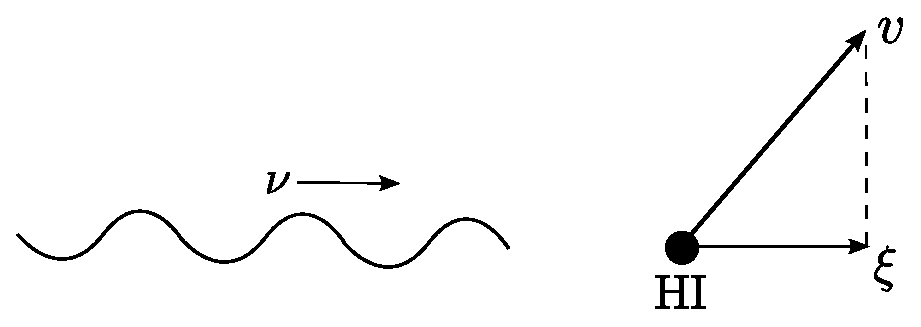
\includegraphics[width=8cm]{dopplerDiagram.eps}
  \caption{This diagram represents the process of Doppler broadening. The HI atom is moving away with velocity $v$ from incoming radiation with frequency $\nu$. The observed frequency of the radiation in the atom's rest frame is $\nu(1-\xi/c)$ where $\xi$ is the component of the velocity parallel with the incident radiation. }
  \label{fig:dopplerDiagram}
\end{figure}


\begin{align}
W(\xi)\dd \xi &= \left( \dfrac{m_p}{2\pi k_{B}T} \right)^{1/2}e^{-m\xi^2/2 k_B T}\dd \xi \\
&= \left(\pi \xi_{0}^{2} \right)^{-1/2} e^{-\xi^{2}/\xi_{0}^{2}} \dd \xi \\
\xi_{0} &\equiv \sqrt{ \dfrac{2k_B T}{m_p}}.
\end{align}

Incident radiation will appear red/blueshifted in the frame of the absorbing atom with the shift being proportional to the atom's velocity \textit{parallel} to the incident radiation, as shown in Figure \ref{fig:dopplerDiagram}. Convolving our line profile with a Maxwell-Boltzmann distribution effectively involves replacing our expression in Eq. \ref{eq:IntroLineProfile} with

{\bf factors of $\lambda_{\alpha}??$}
\begin{align}
\sigma(\nu) &\to \dfrac{\pi e^2}{m_e c}f_{\alpha}\lambda_{\alpha} \int_{-\infty}^{\infty}\dd \xi\ \phi(\nu(1 - \xi/c)) \left(\pi \xi_{0}^{2} \right)^{-1/2} e^{-\xi^2/\xi_{0}^2} \\
&= \dfrac{\pi e^2}{m_e c} \frac{f_{\alpha}}{\pi} \left( \pi \xi_0^2 \right)^{-1/2} \int_{-\infty}^{\infty} \dd \xi \dfrac{(\Gamma/4\pi) e^{-\xi^2/\xi_{0}^{2}}}{(\nu-\nu_{0}(1-\xi/c))^2+(\Gamma/4\pi)^2}. \label{eq:IntroConvolution}
\end{align}

Here, we can make a couple substitutions and redefinitions:

\begin{align}
\Delta v_{\text{D}} &\equiv \nu_{0}\dfrac{\xi_{0}}{c} & y &\equiv -\xi/\xi_0 \\
v &\equiv \dfrac{\nu - \nu_{0}}{\Delta v_{\text{D}}} & a &\equiv \dfrac{\Gamma}{4\pi \Delta v_{\text{D}}}.
\end{align}

The quantity $\Delta v_{\text{D}}$ is known as the ``Doppler parameter" and is the red/blueshift in frequency space that the atom sees due to its thermal motion. The quantity $v$ is just the distance from line center in velocity space in units of the Doppler parameter. The quantity $a \equiv (\Gamma/4\pi)/\Delta v_{\text{D}}$ represents the ratio of the natural line width to the Doppler width. Rewriting our expression in Eq. \ref{eq:IntroConvolution}, we obtain

\begin{align}
\sigma(\nu) &= \dfrac{\pi e^2}{m_e c}f_{\alpha}\dfrac{1}{\sqrt{\pi}\Delta v_{\text{D}}} \dfrac{a}{\pi}\int_{-\infty}^{\infty}\dd y\ \dfrac{e^{-y^2}}{(v-y)^2+a^2}\\ 
&\equiv \dfrac{\sqrt{\pi} e^2}{m_e c} f_{\alpha}\dfrac{H(a,v)}{\Delta v_{\text{D}}}
\end{align}
where $H(a,v)$ is known as the Hjerting function \gloss{Hjerting Function}{Also known as the \textit{Voigt Function}, this function is commonly used in describing line profiles which incorporate Doppler broadening and the natural line width. This function is very relevant when studying the hydrogen damping wing.} or the Voigt function\gloss{Voigt Function}{Also known as the \textit{Hjerting Function}, this function is commonly used in describing line profiles which incorporate Doppler broadening and the natural line width. This function is very relevant when studying the hydrogen damping wing.}. So finally, we have obtained an expression for the \lya\ line profile incorporating the natural line width and Doppler broadening. The profile is complex, but nonetheless, it contains information about the gas temperature and, given an observation of an absorption line, we should be able to perform fits to this profile in order to infer the temperature of the IGM.

In Figure \ref{fig:QuasarProximityTemp}, \cite{BoltonQuasar} look for \lya\ absorption lines in the proximity zones of high-redshift quasars in order to fit for the associated Doppler parameter and make inferences about the temperature. The top panel shows the fractional transmission for a mock quasar spectrum. The dashed curves indicate regions where absorption-line fitting was carried out and the vertical arrows indicate where the line centers were found from the fits. The second and third panel show the underlying temperature and density field, respectively. The bottom panel shows the true spectrum in question along with the same information regarding the line profile fits. These authors were able to use these fits to make inferences about the temperature of the IGM nearby the quasar. From these temperature measurements, and through utilizing Eq. \ref{eq:dtdt}, these authors were able to place interesting limits on the ending of reionization ($z_{\text{H}} <  9$ assuming that the quasar reionizes its vicinity and Pop II stars drive reionization). This specific measurement is very difficult, however. The argument is essentially that the inferred temperature of the gas is too hot for reionization to have ended long before $z = 9$, otherwise the gas would have had more time to cool below the measured temperature. However, the regions nearby quasars should see a significantly-enhanced ionization field and all constraints made from measurements within this region hinge on ones ability to accurately account for such effects. 


The aforementioned technique for measuring the temperature is useful, but has the drawback that it requires a certain level of transmission in the quasar spectra in order to confidently fit a single absorption-line profile. However, at $z > 5$, individual absorption features blend together and the forest becomes somewhat inverted where, instead of stretches of transmission being punctuated with absorption features, stretches of absorption are punctuated with transmission features. this renders the goal of fitting for individual Voigt profiles impossible in the IGM. This also explains why \ref{BoltonQuasar} analyze the nearby a high-redshift quasar, where the transmission is enhanced due to the strengthened ionization field. 

Zaldarriaga (2002), Theuns \& Zaroubi (2000)

{\bf we may want to look for a more detailed explanation of the $\frac{\dd T}{\dd t}$ expression. }

This procedure has been applied to measure the temperature of the IGM at a variety of redshifts ({\bf cites}). Alternatively, Lidz {\bf cite} proposed using Morlet wavelet analysis as a measure of small-scale structure which is also indicative of the temperature. However, these analyses all depend on the \lya\ forest having significant transmission. While this is true for $z < 5$, for $z > 5$ the picture is flipped long periods of absorption are punctuated by some transmission. 

 
% Maybe we can defer discussion of this equation to chapter 3?
\begin{align}
\dfrac{\dd T}{\dd t} &= -2HT + \dfrac{2T}{3(1+\delta)}\dfrac{\dd \delta}{\dd t} + \dfrac{T}{\mu} \dfrac{\dd \mu}{\dd t} + \dfrac{2\mu m_p}{3\rho k_B}(\mathcal{H} - \Lambda) \label{eq:dtdt}
\end{align}

\begin{figure}[h]
  \centering
  \includegraphics[width=11cm]{BoltonIGMTemperature_Fig2.ps}
  \includegraphics[width=11cm]{BoltonIGMTemperature_Fig2b.ps}
  \caption{This figure shows mock spectra, and corresponding simulated IGM properties, from \cite{BoltonQuasar} in the top four panels. The bottom panel shows the observed spectrum from SDSS J0818+1722, which \cite{BoltonQuasar} use in order to make temperature measurements inside the proximity zone. Dashed lines indicate regions where Voigt-profile fitting was performed and downward arrows indicate the detected centers of the Voigt profiles.}
  \label{fig:QuasarProximityTemp}
\end{figure}


One option here is to structure this section saying that people typically use something related to the Doppler widths in order to infer the temperature. However, at $z \gtrsim 5$, the forest becomes so absorbed that it inverted, in a sense: long periods of saturated absorption are punctuated with transmission spikes rather than the other way around. This makes Voigt-profile fitting impossible. This has kind of been a problem in measuring the temperature of the $z \gtrsim 5$ IGM, with some people using proximity zones of quasars. These are probably pretty special regions, though, hard to back out information on the IGM as a whole. However, Lidz is a boss and knows how to do it. ({\bf this should be described be 0909.5210}) 


\subsection{The 21-cm Line}
\subsection{The Cosmic Microwave Background}
\subsection{\lya\ Emitters}
\subsection{Luminosity Function Measurements}

\section{Where We Stand}

\begin{enumerate}
\item Bouwens et al. (2015) might be good to include here. Strengthens argument that galaxies reionized the Universe and that quasars/AGN did not.
\end{enumerate}
% ----------------------------------------------------------------------



